\documentclass[12 pt]{article}

\title{Project Synopsis}
\date{12 july, 2015}
\author{R. K yadav}



\maketitle
\tableofcontents
\newpage
\pagenumbering{alph}



\begin{document}

\section{Introduction}
Today, was not goog for me. today i work on image processing . But i can'y find functions of image processing .this is not my fault. Actually there was no any function of image processing. So i do the c++ . I create program of c++ regarding bank balance. THis program ask for account no and bank balance of user . After it ask for deposit amount and withdraw amount . swicth() function is used in this for making choice. After proceeding the choice, it display current balance after deduction or addition. now i am doing Latex i am creating a article in latex.
  
\subsection{image processing}
I am doing image processing in octave.For doing this i am using various functions of image processing. Octave-forge package is used for this.

\subsection{c++}
There are various module in project.this is article that contain a various sections.

\subsection{latex} 
i am using a latex.

\newpage
\section{Module}
There are various module taht are implemented foe creating ptoject.These are--

\subsection{CSS}
this is a style sheet tat control the overall design of page.
\subsection{javascript}
it is a scripting language. it create a interactive page.

    \documentclass[10pt,a4paper]{article}
    \usepackage[T1]{fontenc}
    \usepackage{tikz}

    \begin{document}
      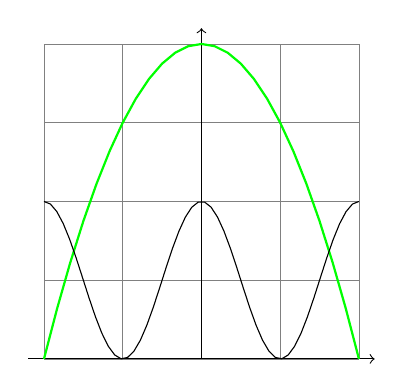
\begin{tikzpicture}
        \draw[help lines] (-2,0) grid (2,4);
        \draw[->] (-2.2,0) -- (2.2,0);
        \draw[->] (0,0) -- (0,4.2);
        \draw[green, thick, domain=-2:2] plot (\x, {4-\x*\x});
        \draw[domain=-2:2, samples=50] plot (\x, {1+cos(pi*\x r});
      \end{tikzpicture}
      \begin{tikzpicture}[domain=0:4]
        \draw[very thin,color=gray] (-0.1,-1.1) grid (3.9,3.9);
        \draw[->] (-0.2,0) -- (4.2,0) node[right] {$x$};
        \draw[->] (0,-1.2) -- (0,4.2) node[above] {$f(x)$};
        \draw[color=red]    plot (\x,\x)             node[right] {$f(x) =x$};
        \draw[color=blue]   plot (\x,{sin(\x r)})    node[right] {$f(x) = \sin x$};
       
    \end{document}

\end{document}
